\documentclass[pdf]{beamer}
\usepackage[]{hyperref,graphicx,siunitx,natbib,lmodern}
%\usepackage[clean,inkscape={inkscape -z -D}]{svg}
%\mode<presentation>{\usetheme{Warsaw}\usecolortheme{beaver}}
\usepackage{willamette}

\bibliographystyle{unsrt}
\renewcommand{\bibsection}{\subsubsection*{\bibname } }

%preamble
\title[Supersonic Baseballs]{Supersonic Baseballs: Characterization and Analysis of Near-Earth Meteoroids via Lunar Impact Observations}
\subtitle{}
\author{Jed Rembold\inst{1}}
\institute{
  \inst{1}
  Willamette University\\
  Salem, OR
}
\date{Sept 25, 2015}

\begin{document}

\frame{\titlepage}

%\begin{frame}{Table of Contents}
%  \tableofcontents
%\end{frame}

\section{Introduction}

\begin{frame}{General Interests}
  \begin{columns}
	\column{.5\textwidth}
	\begin{itemize}
	  \item Astrophysics
	  \item Optical Observations
		\begin{itemize}
		  \item Small asteroids
			\begin{itemize}
			  \item Too small to be detected by other means
			  \item Burn up in Earth's atmosphere
			  \item Rocky in nature (not icy)
			\end{itemize}
		\end{itemize}
	\end{itemize}
	\column{.5\textwidth}
	\begin{figure}[h!]
	  \centering
	  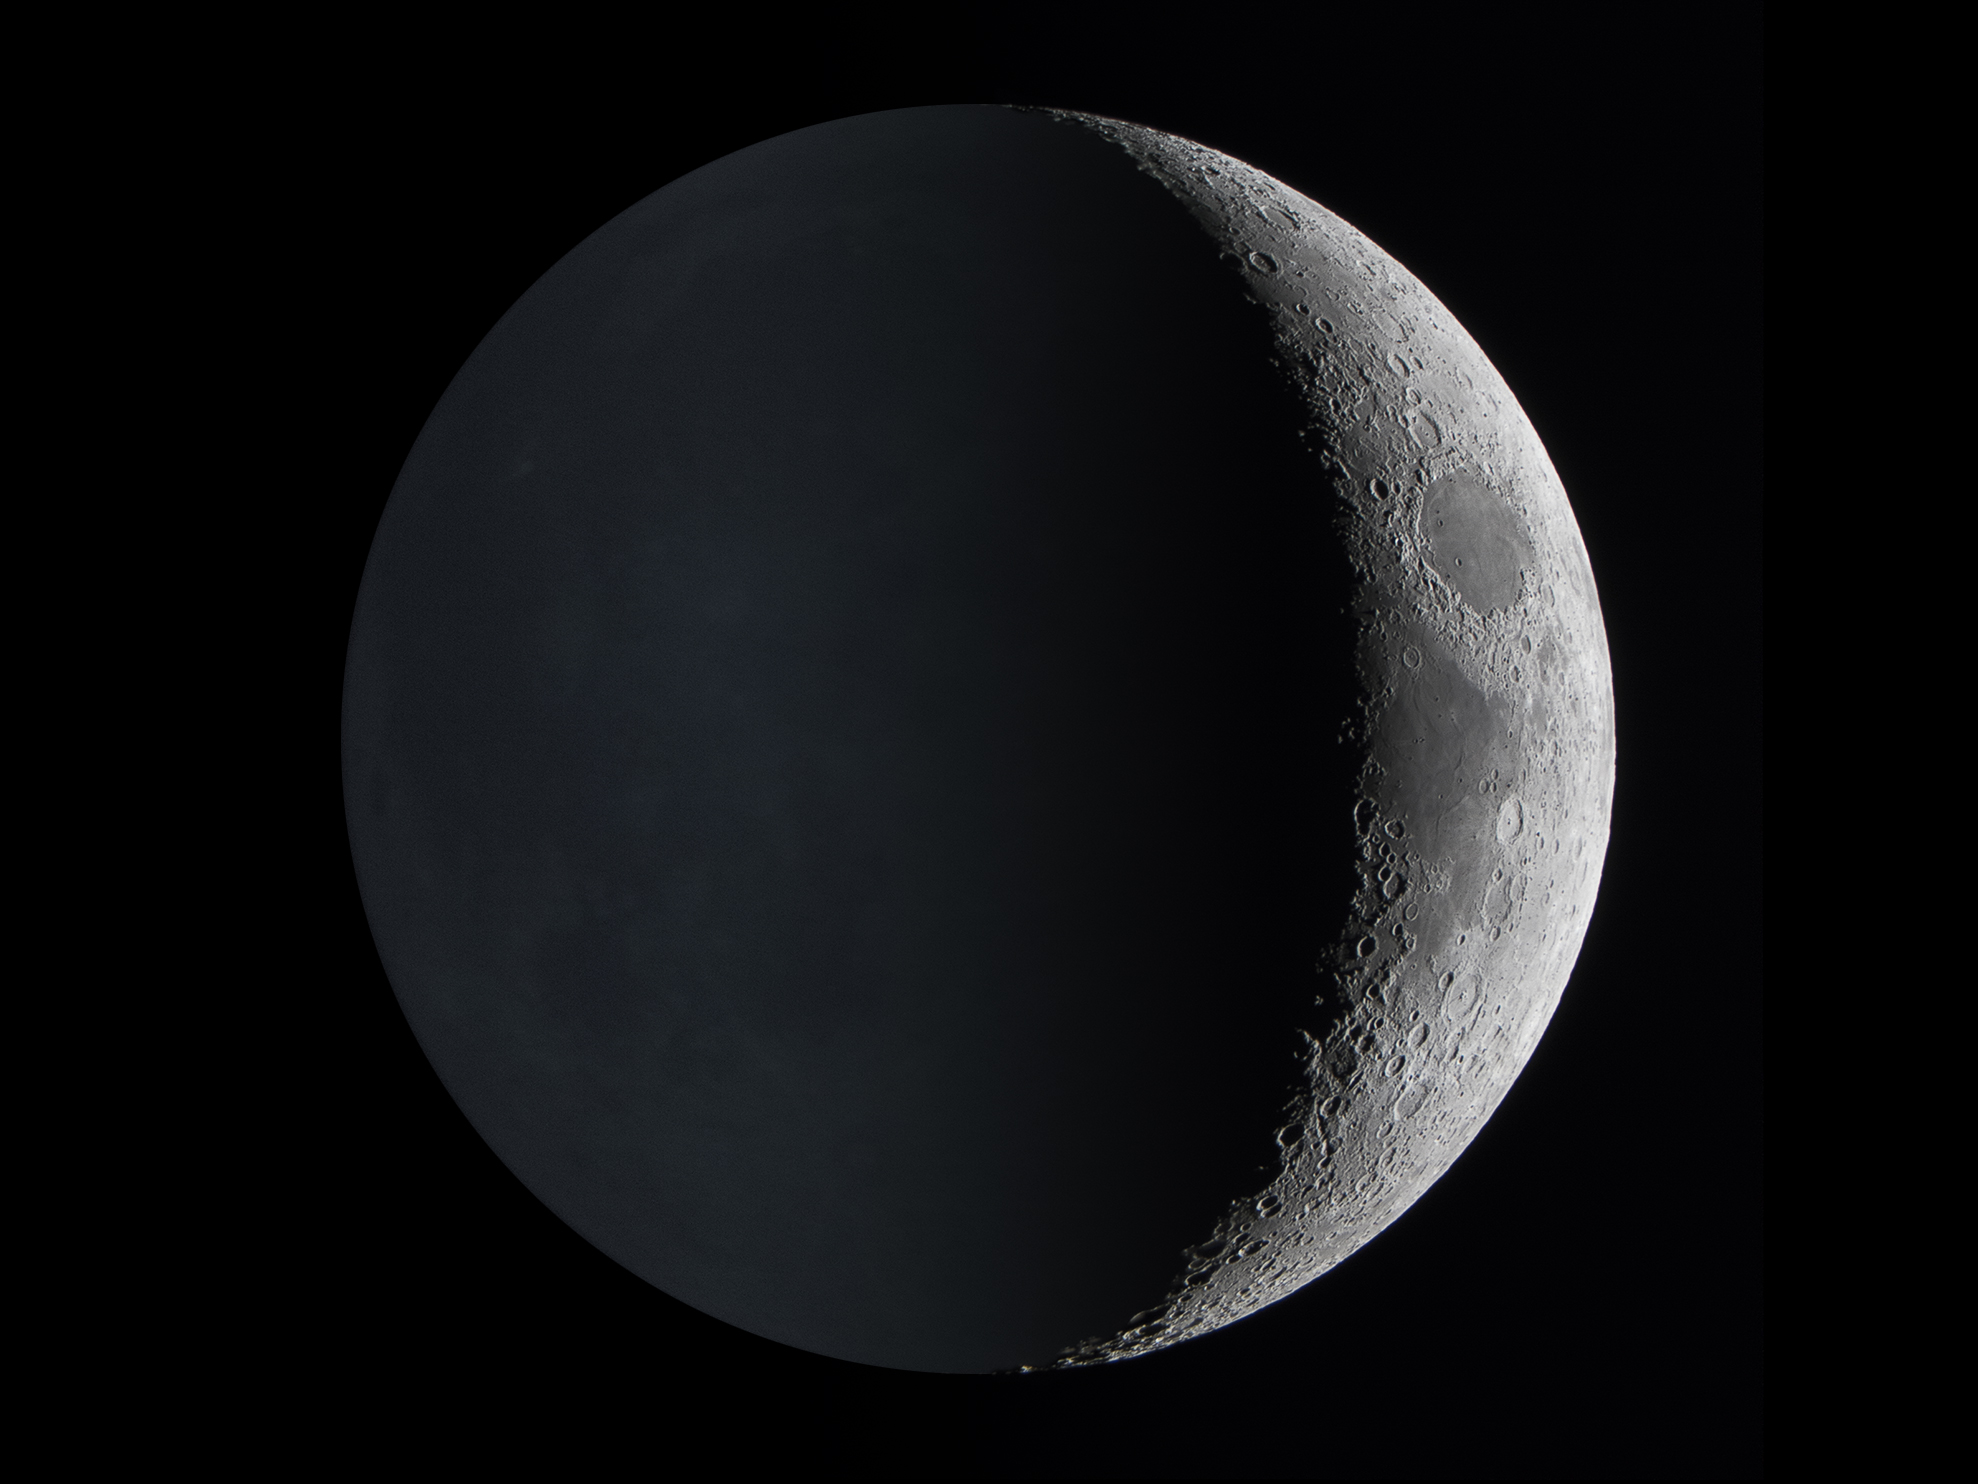
\includegraphics[width=\textwidth]{Images/EarthShine.jpg}
	\end{figure}
  \end{columns}
\end{frame}

\begin{frame}{Goals}
  To utilize the night portion of the lunar surface as a giant detection screen upon which the optical flashes caused by small asteroids striking the surface can be observed in order to obtain an average flux rate for small impactors.
  \begin{columns}
	\column{.5\textwidth}
	\begin{block}{Pros}
	  \begin{itemize}
		\item Massive amount of available observable area (9-15 million square kilometers)
		\item Even tiny objects are bright when they smash things going really fast
	  \end{itemize}
	\end{block}
	\column{.5\textwidth}
	\begin{block}{Cons}
	  \begin{itemize}
		\item Limited observing times
		  \begin{itemize}
			\item Lunar Phases
			\item Daytime lunar transits
		  \end{itemize}
		\item False Positives
		  \begin{itemize}
			\item Airplanes/Satellites
			\item Cosmic Rays
		  \end{itemize}
	  \end{itemize}
	\end{block}
  \end{columns}
\end{frame}

\begin{frame}{Why look at these things?}
  \begin{itemize}
	\item Meteors are damaging!
	  \begin{itemize}
		\item Chelyabinsk energy = 20-30 atomic bombs
		\item Smaller meteors still go really fast (\SIrange{17}{66}{\kilo\meter\per\second}) (Think a baseball at nearly Mach 200!)
		\item Small = harder to detect
	  \end{itemize}
	\item Better understanding = Better risk analysis
	\item Solar System Evolution
	  \begin{itemize}
		\item Collisions and Accretion - small debris is very important!
	  \end{itemize}
  \end{itemize}
\end{frame}


\subsection{Background}
\begin{frame}{Background: The Beginnings}
  \begin{itemize}
	\item Curiosity about lunar impacts not new (Gordon in 1921) \citep{Gordon1921}
	\item Detecting them has taken much longer
	  \begin{itemize}
		\item ``Hey, I just saw a flash on the lunar surface!''\par\hspace{1cm} --Harrison Schmitt, Apollo 17, 1972 \citep{NASA1972}
		\item In 1993, Melosh theorized that rocky debris down to 1 meter should be visible given typical equipment of the time \citep{Melosh1993}
		\item First observed and confirmed during the 1999 Leonid meteor shower by Ortiz and Dunham \citep{Ortiz2000}
	  \end{itemize}
  \end{itemize}
\end{frame}

\begin{frame}{Background: Onward to the Present!}
  \begin{itemize}
	\item Meteor Showers easiest to observe
	  \begin{itemize}
		\item Seen again in 2001 Leonids shower by Ortiz and Cudnik \citep{Ortiz2002,Cudnik2003}
		\item First seen in 2004 Perseid shower by Yanagisawa \citep{Yanagisawa2006}
	  \end{itemize}
	\item Also seen outside of meteor showers
	  \begin{itemize}
		\item Called Sporadics
		\item First reported by Ortiz between 2001-2004 \citep{Ortiz2006}
	  \end{itemize}
	\item NASA's Marshall Space Flight Center (MSFC) began observations around 2005 \citep{Cooke2007}
  \end{itemize}
\end{frame}

\begin{frame}{Background: Energetics}
  \begin{columns}
	\column{0.5\textwidth}
	\begin{itemize}
	  \item Only a percentage of kinetic energy converted to visible light (luminous efficiency)
	  \item Not well determined
		\begin{itemize}
		  \item Ortiz modeled off observed to expected impact rate \citep{Ortiz2002}
		  \item Sigismondi estimated from thermodynamic principles \citep{Sigismondi2001}
		  \item Swift and Moser used the above and gas gun experiments \citep{Swift2011}
		\end{itemize}
	\end{itemize}
	\[\eta(v) = 1.5\times 10^{-3} e^{-(\SI{9.3}{\kilo\meter\per\second})^2/v^2}\]
	\column{0.5\textwidth}
	\begin{figure}[h!]
	  \centering
	  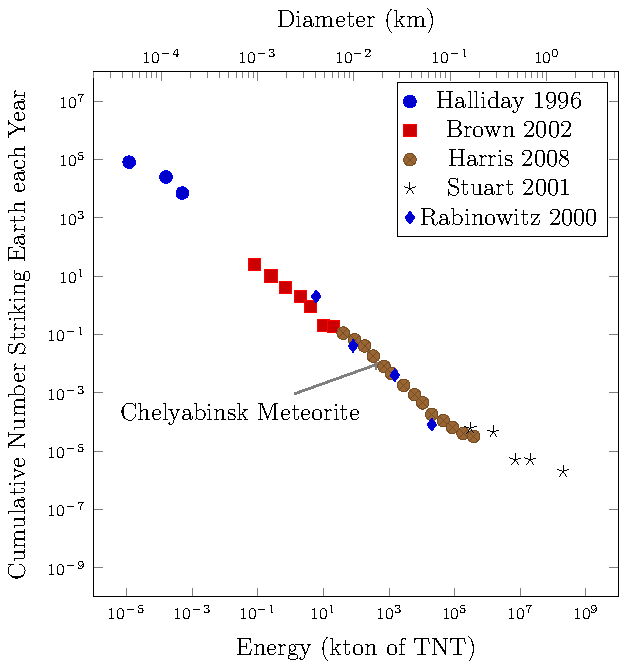
\includegraphics[width=\textwidth]{Images/Cumulative-Flux-2-Date_V2.pdf}
	\end{figure}
  \end{columns}
\end{frame}

\section{Methods}

\subsection{Basics}

 \begin{frame}{Outline}
   \tableofcontents[currentsection]
 \end{frame}

\begin{frame}{Observational Setup}
  \begin{figure}[ht!]
	\centering
	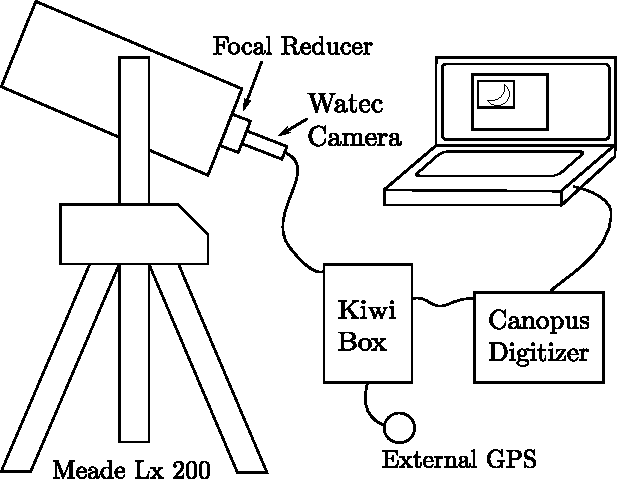
\includegraphics[width=.75\textwidth]{Images/equipment_setup2.pdf}
  \end{figure}
\end{frame}

\begin{frame}{Field of View}
  \begin{figure}[h!]
	\centering
	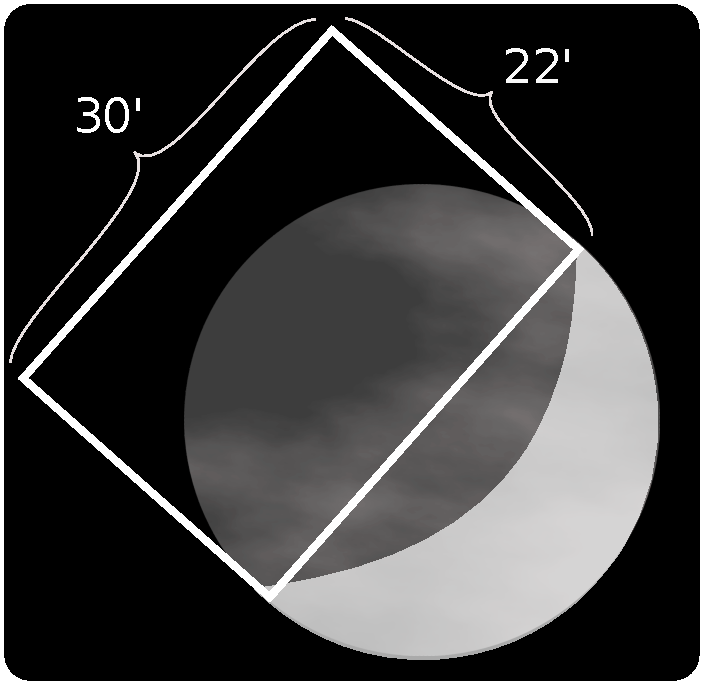
\includegraphics[width=.65\textwidth]{Images/fieldofview2.pdf}
  \end{figure}
\end{frame}

\begin{frame}{LunarScan}
  \begin{figure}[ht!]
	\centering
	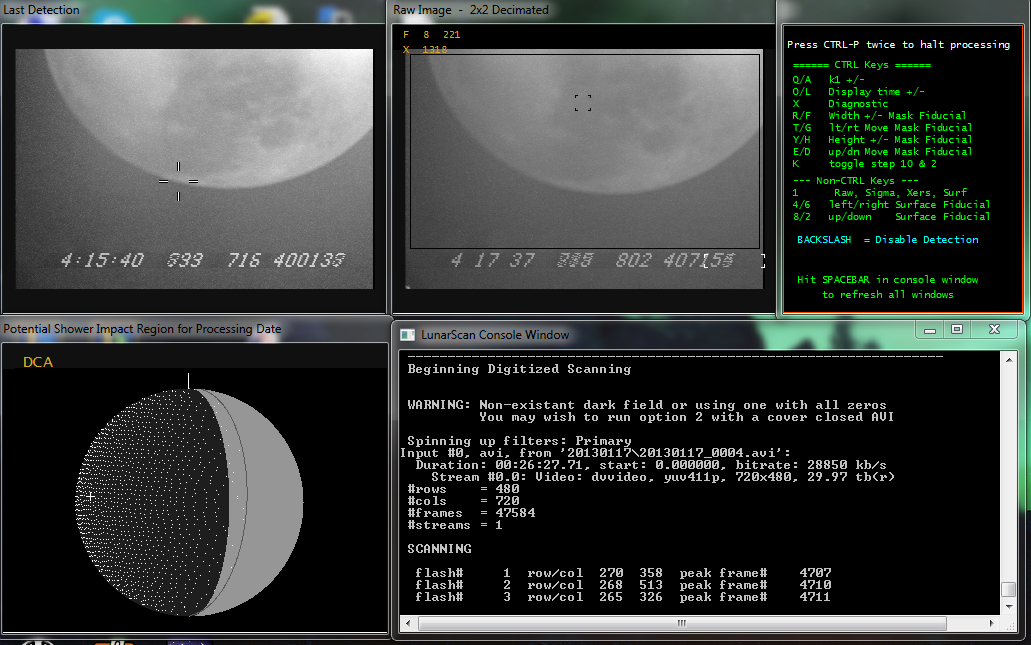
\includegraphics[width=\textwidth]{Images/LunarScan_screenshot.png}
  \end{figure}
\end{frame}

\begin{frame}{LunarScan Example}
  \begin{figure}[h!]
	\centering
	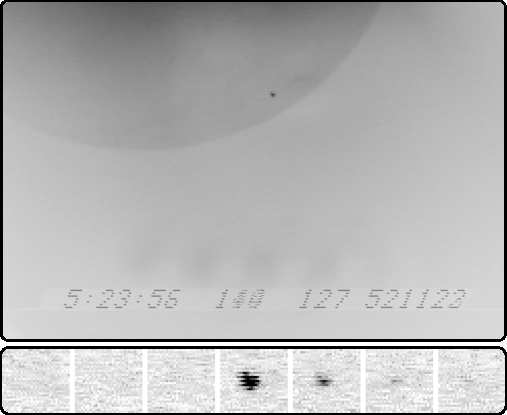
\includegraphics[width=.75\textwidth]{Images/lunarscan_example.pdf}
  \end{figure}
\end{frame}

\begin{frame}{Magnitude Calibration}
  \begin{columns}
	\column{.5\textwidth}
	\begin{itemize}
	  \item Open Filter for sensitivity
		\begin{itemize}
		  \item $\Rightarrow$ Calibrated to $R$ band
		\end{itemize}
	  \item LiMovie used for photometry
	  \item AviSynth used for video decoding
	\end{itemize}
	\column{.5\textwidth}
	\begin{figure}[ht!]
	  \centering
	  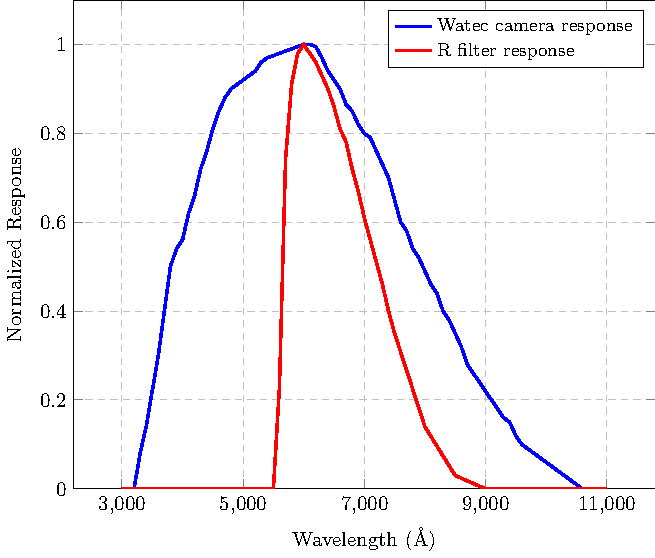
\includegraphics[width=\textwidth]{Images/SensorResponses.pdf}
	\end{figure}
  \end{columns}
  \[m_{act} = -2.5\log(g) - C_{offset} - kx - T(B-V)\]
 \end{frame}

 \begin{frame}{Impact Color Correction}
   \begin{columns}
	 \column{.5\textwidth}
	 \begin{figure}[ht!]
	   \centering
	   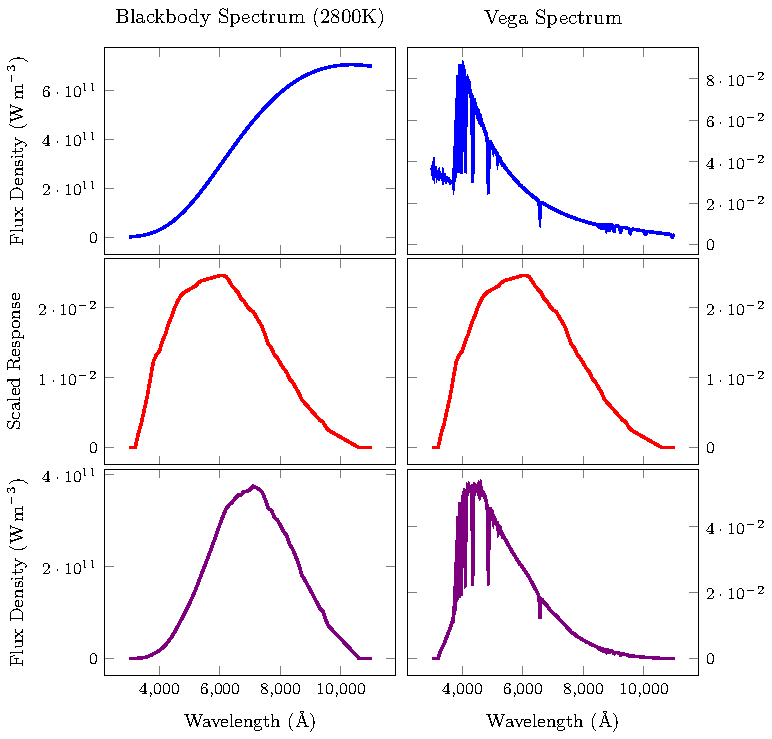
\includegraphics[width=\textwidth]{Images/Convolve_Example.pdf}
	 \end{figure}
	 \column{.5\textwidth}
	 \[m_{imp} = m_{vega} - 2.5\log\left( \frac{f_{imp}}{f_{vega}} \right)\]
	 \begin{figure}[ht!]
	   \centering
	   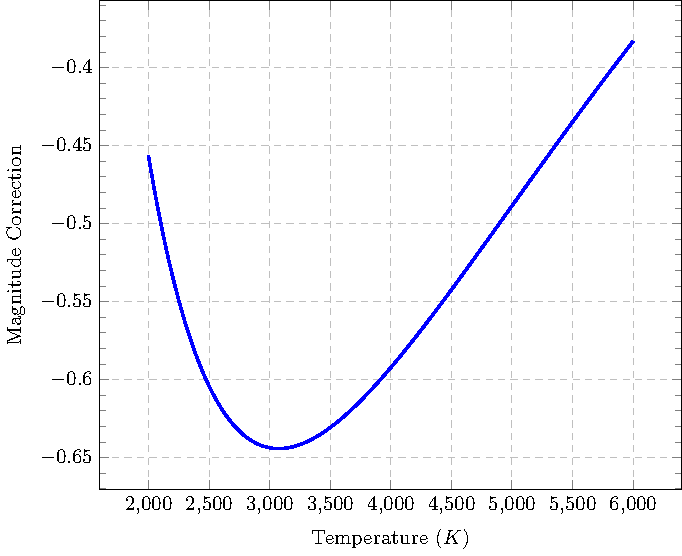
\includegraphics[width=\textwidth]{Images/REx_Correction.pdf}
	 \end{figure}
   \end{columns}
 \end{frame}

 \subsection{Energetics}

 \begin{frame}{Magnitude to Energy}
   \begin{columns}
	 \column{.5\textwidth}
	 \begin{itemize}
	   \item Flux Density (\si{\watt\per\centi\meter^2\per\angstrom}):
		 \[f_{\lambda} = 10^{-7}\cdot 10^{-(R+21.1+0.555)/2.5}\]
	   \item Avg Flux (\si{\watt\per\centi\meter^2}):
		 \[f = \Delta \lambda f_\lambda\]
	 \end{itemize}
	 \column{.5\textwidth}
	 \begin{itemize}
	   \item Luminosity (\si{\watt}):
		 \[L = \frac{\eta (KE)}{\Delta t}\]
	   \item Flux $\rightarrow$ Luminosity:
		 \[f = \frac{L}{2\pi d^2}\]
	 \end{itemize}
   \end{columns}
   \begin{block}{Impactor Kinetic Energy}
	 \[KE = \frac{2\pi d^2 f_\lambda \Delta \lambda \Delta t}{\eta}\]
   \end{block}
 \end{frame}

 \subsection{Supplementary Octave Work}

 \begin{frame}{Observed Lunar Area}
   \begin{columns}
	 \column{.5\textwidth}
	 \begin{figure}[ht!]
	   \centering
	   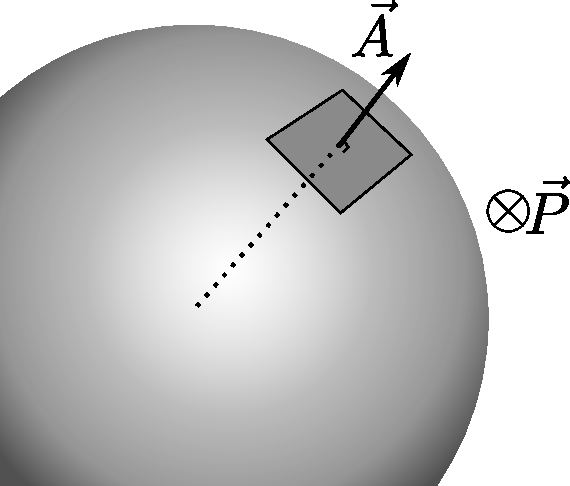
\includegraphics[width=\textwidth]{Images/lunararea1.pdf}
	 \end{figure}
	 \column{.5\textwidth}
	 \begin{figure}[ht!]
	   \centering
	   
\includegraphics[width=\textwidth]{Images/lunararea_example.pdf}
	 \end{figure}
   \end{columns}
 \end{frame}

 \begin{frame}{Selenographic Latitude and Longitude}
   \begin{columns}
	 \column{.5\textwidth}
	 \begin{figure}[ht!]
	   \centering
	   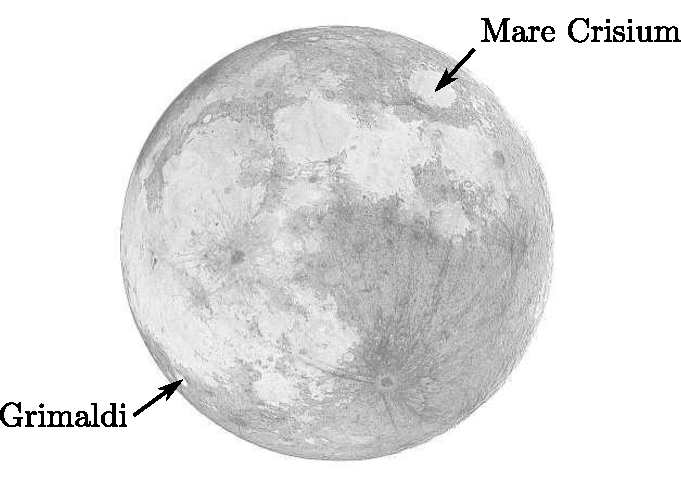
\includegraphics[width=\textwidth]{Images/reference_craters.pdf}
	 \end{figure}
	 \column{.5\textwidth}
	 \begin{figure}[ht!]
	   \centering
	   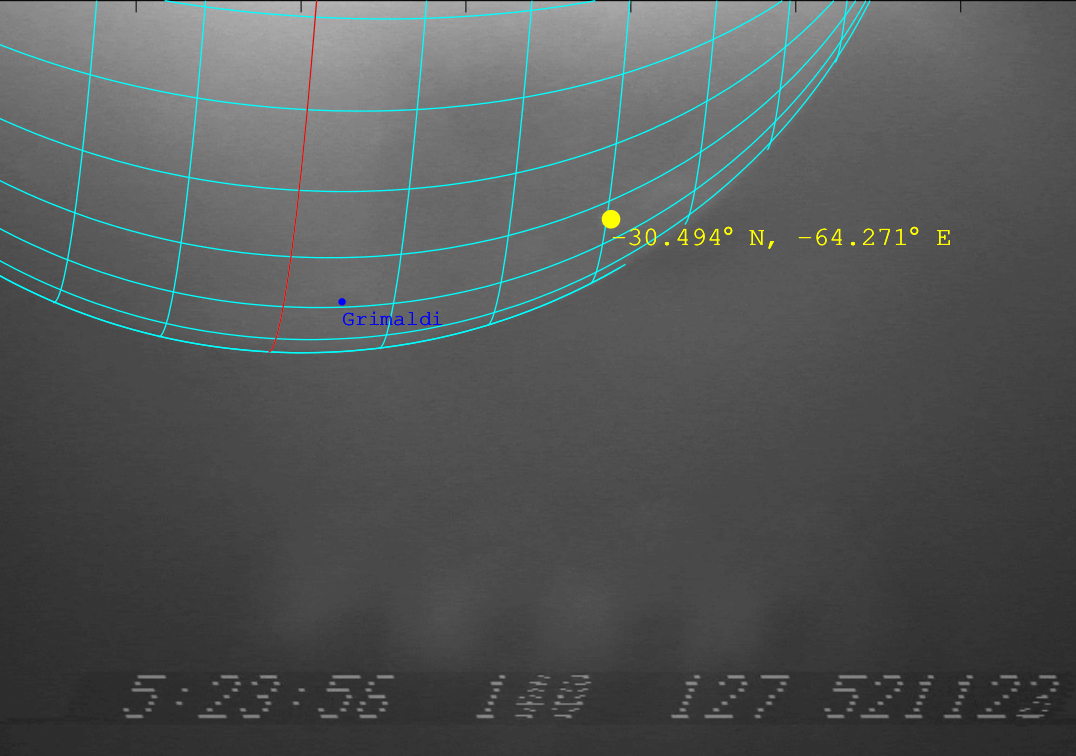
\includegraphics[width=\textwidth]{Images/coord_fits.png}
	 \end{figure}
   \end{columns}
 \end{frame}

 \begin{frame}{Analysis Command}
   \begin{figure}[h!]
	 \centering
	 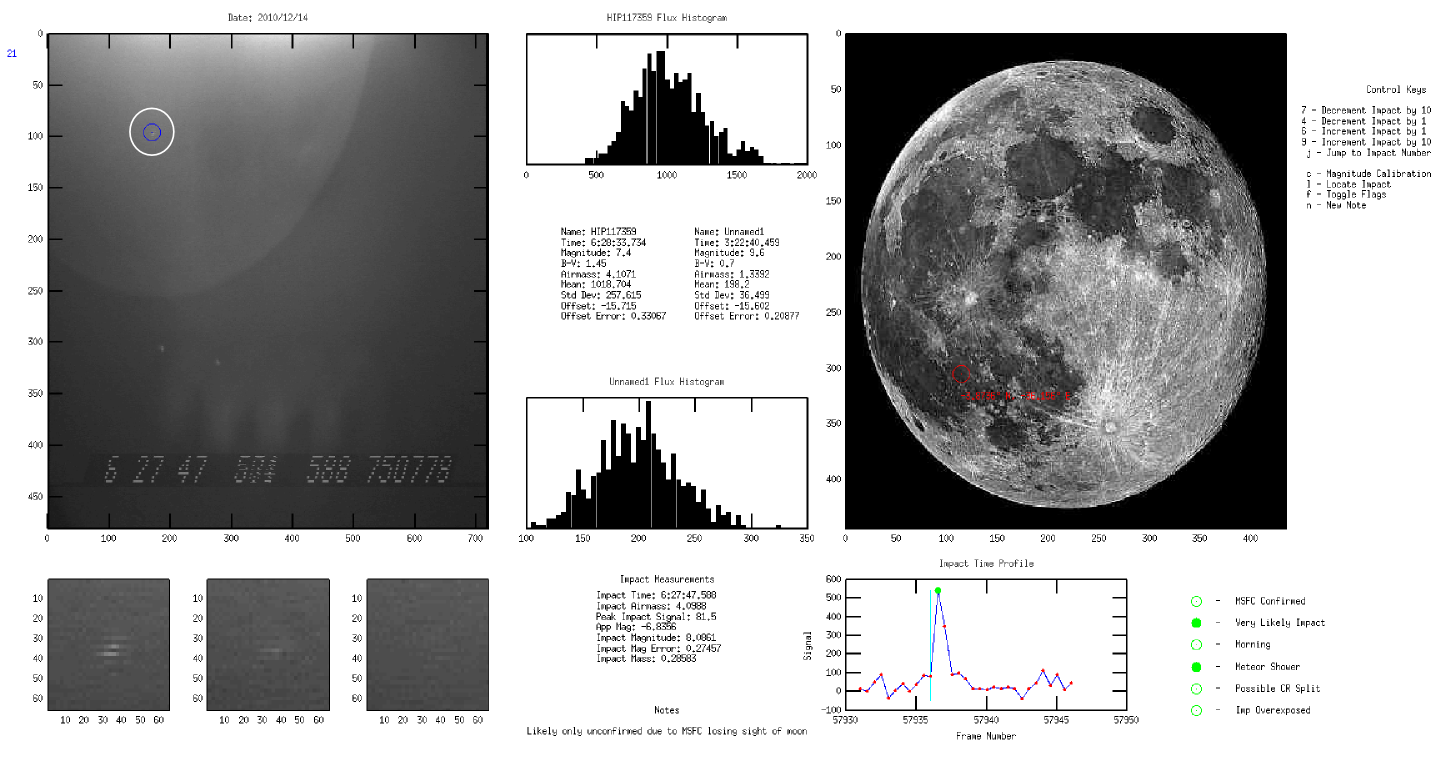
\includegraphics[width=\textwidth]{Images/viewer.png}
   \end{figure}
\end{frame}

 \section{Data}

 \subsection{Accepted Impacts}

 \begin{frame}{Outline}
   \tableofcontents[currentsection]
 \end{frame}

 \begin{frame}{False Positives}
   \begin{columns}
	 \column{.5\textwidth}
	 \begin{itemize}
	   \item False Positives
		 \begin{itemize}
		   \item Streaks/Movement
		   \item Doubles/Splits
		   \item Overexposure
		 \end{itemize}
	   \item Positive Signs
		 \begin{itemize}
		   \item Extended time signature
		 \end{itemize}
	 \end{itemize}
	 \begin{figure}[ht!]
	   \centering
	   
\includegraphics[width=1.45\textwidth]{Images/ExtImpSeq.pdf}
	 \end{figure}
	 \column{.5\textwidth}
	 \begin{figure}[ht!]
	   \centering
	   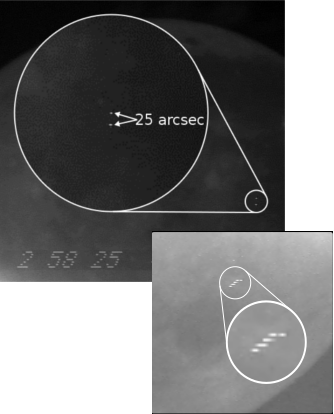
\includegraphics[width=.8\textwidth]{Images/false_positives.png}
	 \end{figure}
   \end{columns}
 \end{frame}

 \begin{frame}{Accepted Impacts}
   \begin{figure}[ht!]
	 \centering
	 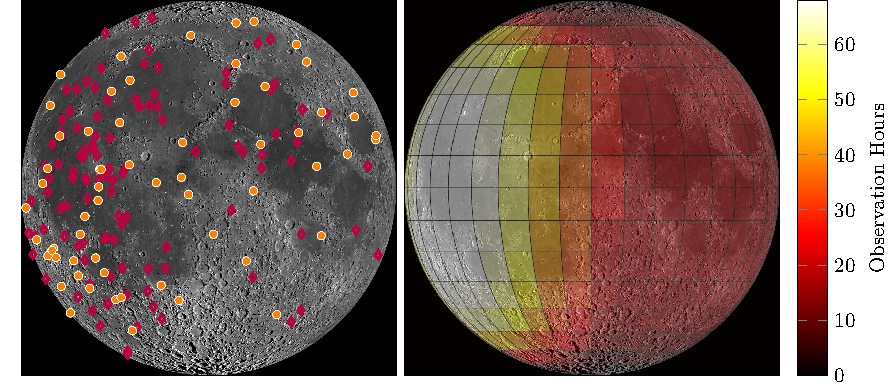
\includegraphics[width=1.05\textwidth]{Images/Impacts_and_Bias.pdf}
   \end{figure}
 \end{frame}

 \subsection{Completeness Limit}

 \begin{frame}{The Completeness Limit}
   \begin{columns}
	 \column{.5\textwidth}
	 \begin{itemize}
	   \item Dimmer impacts likely not fully sampled
	   \item Expect to see increasingly more small/dim impacts
	   \item Turnover indicates completeness limit
	   \item Taken to correspond to magnitude 8.5
	 \end{itemize}
	 \column{.5\textwidth}
	 \begin{figure}[ht!]
	   \centering
	   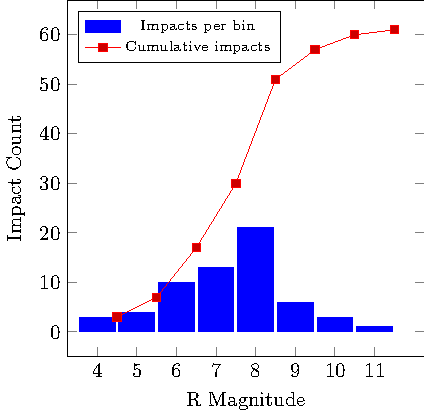
\includegraphics[width=\textwidth]{Images/RMagHist.pdf}
	 \end{figure}
   \end{columns}
 \end{frame}


 \section{Results}

 \begin{frame}{Outline}
   \tableofcontents[currentsection]
 \end{frame}

 \begin{frame}{Impact Flux Rate}
   \begin{itemize}
	 \item Average flux rate computed to the completeness limit
	   \[\frac{\SI{51}{Impacts}}{\left( \SI{5.77E6}{\kilo\meter^2} \right)\left( \SI{80.97}{\hour} \right)} = \left( 1.09\pm0.02 \right)\times 10^{-7} \si{\kilo\meter^{-2}\hour^{-1}}\]
	 \item Slightly higher than MSFC latest value of \SI{1.03E-7}{\kilo\meter^{-2}\hour^{-1}} to 9th magnitude \citep{Suggs2014}
	 \item Corresponds to 9-17 impact difference between databases
	 \item Plausible over multi-year observations with highly variable impact rates, observing times, and conditions
   \end{itemize}
 \end{frame}

 \subsection{Flash Variations}

 \begin{frame}{Flash Variations}
   \begin{columns}
	 \column{.5\textwidth}
	 \begin{itemize}
	   \item Photometric evolution may describe unknown impact parameters
		 \begin{itemize}
		   \item Impacter composition?
		   \item Impacted terrain composition?
		   \item Impact angle?
		 \end{itemize}
	   \item Many variables, tough to analyze with limited dataset
	 \end{itemize}
	 \column{.5\textwidth}
	 \begin{figure}[ht!]
	   \centering
	   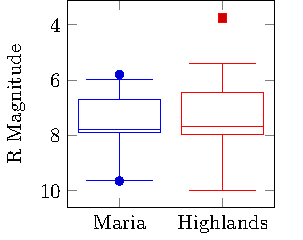
\includegraphics[width=\textwidth]{Images/LunarLightDarkBoxplot.pdf}
	 \end{figure}
   \end{columns}
 \end{frame}

 \subsection{Energy Distribution}

 \begin{frame}{Energy Distribution: The Initial State}
   \begin{figure}[ht!]
	 \centering
	 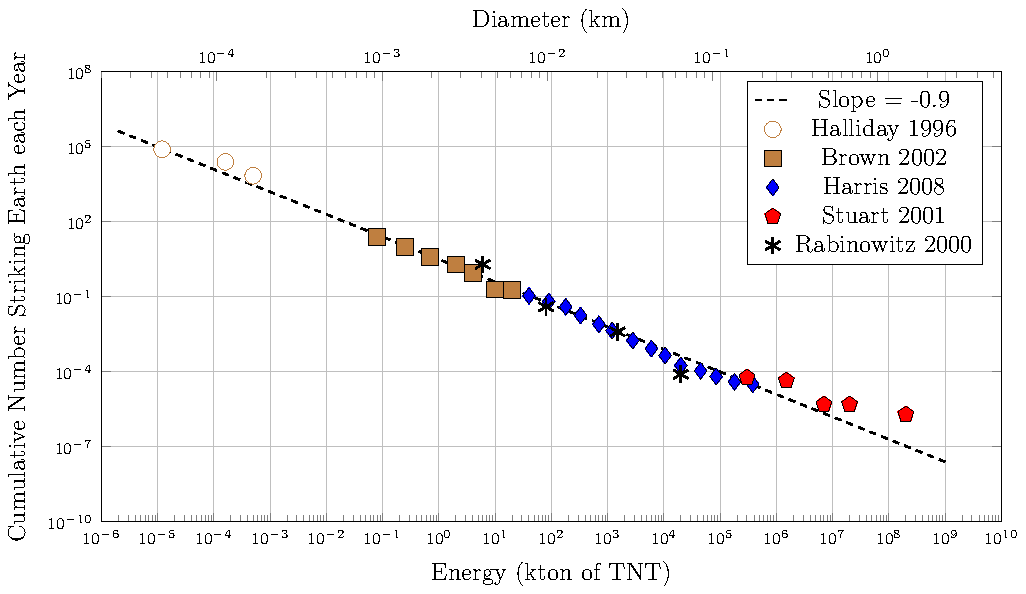
\includegraphics[width=\textwidth]{Images/Cumulative_Flux_All_1.pdf}
   \end{figure}
 \end{frame}
 
 \begin{frame}{Energy Distribution: State this Spring}
   \begin{figure}[ht!]
	 \centering
	 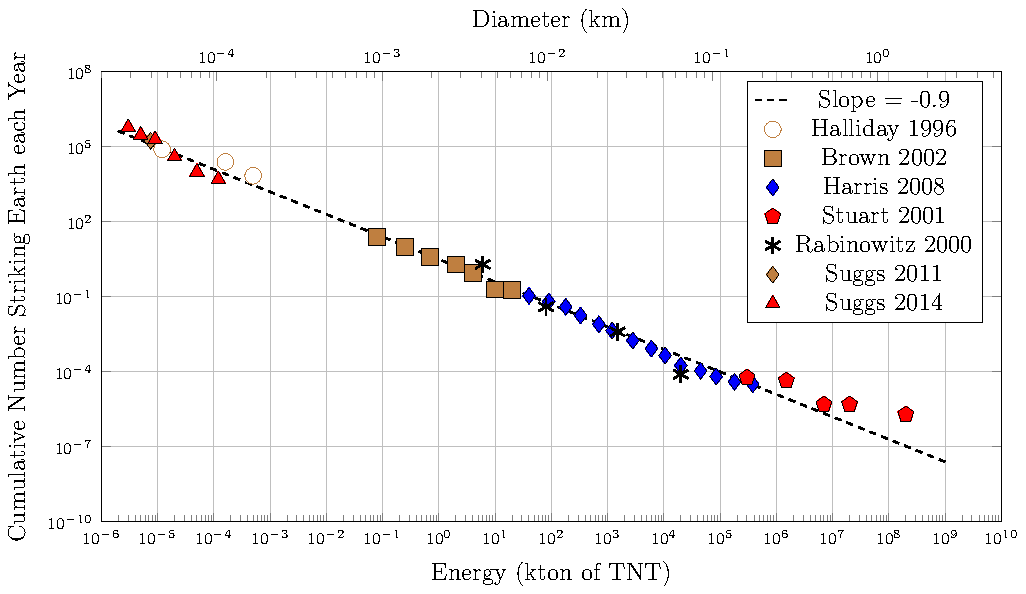
\includegraphics[width=\textwidth]{Images/Cumulative_Flux_All_2.pdf}
   \end{figure}
 \end{frame}
 
 \begin{frame}{Energy Distribution}
   \begin{figure}[ht!]
	 \centering
	 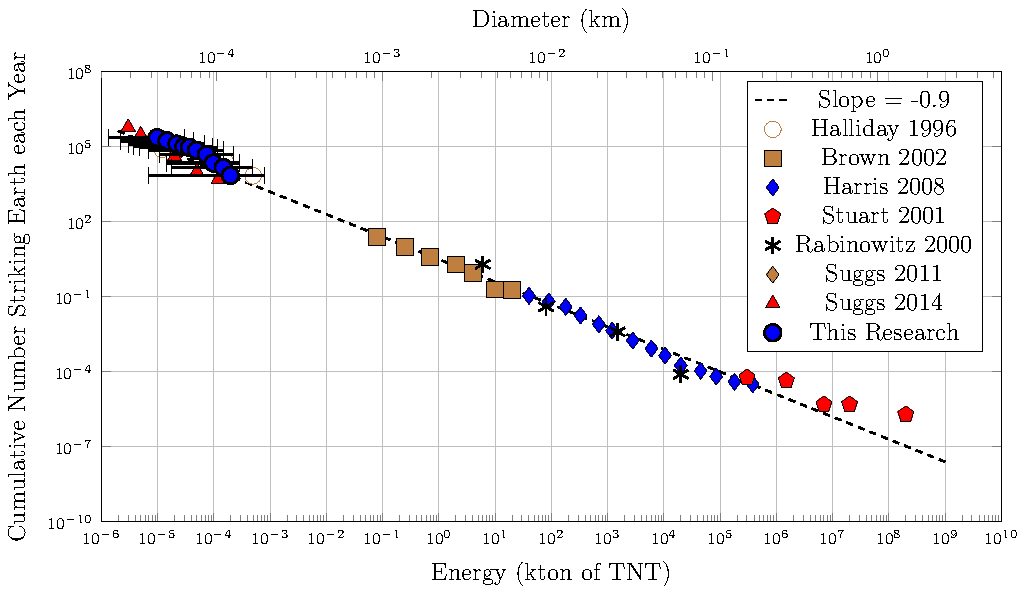
\includegraphics[width=\textwidth]{Images/Cumulative_Flux_All_3.pdf}
   \end{figure}
 \end{frame}

 \section{Conclusions}

 \subsection{Conclusions}

 \begin{frame}{Conclusions: Primary Purpose}
		To assemble and devise a lunar impact experimental setup capable of observing many lunar impacts over a prolonged time in order to estimate a small debris flux rate near Earth
		\begin{block}{Result}
			An experimental setup and analysis pipeline was devised and created which observed 61 accepted lunar impacts over 80 hours of observation between 2010 and 2012. Average impact flux rates to magnitude 8.5 measured \SI{1.09E-7}{impact\per\kilo\meter^2\per\hour}, corresponding to approximately 1 lunar strike every 30 minutes.
		\end{block}
 \end{frame}

 \begin{frame}{Conclusions: Secondary Purposes}
		To investigate relationships between impact brightness, speed, composition, and impacted terrain
		\begin{block}{Result}
		  Lunar terrain composition seems to play only a small role in the luminous efficiency, though a larger dataset is needed
		\end{block}
		To estimate an energy distribution for small size debris near Earth
		\begin{block}{Result}
		  There is no deviation within error bars from the power law governing the energy distribution of larger asteroids
		\end{block}
\end{frame}

 \begin{frame}{Future/Current Work}
   \begin{itemize}
	 \item Working to setup an all-sky camera for fireball detection (with Kyle)
	 \item Fireballs can be analyzed for both orbital information and energetic population density
	 \item Working on code for automatic (hopefully) real-time detection of fireballs/lunar impacts
	 \item Rewritting much of lunar impact analysis code into Python for future ease of use and better automation
   \end{itemize}
 \end{frame}

 \begin{frame}{Acknowledgments}
   I'd like to take a moment to thank the following people:
   \begin{itemize}
	 \item Eileen Ryan, for her patience, support, and insight
	 \item Bill Ryan, for originally conceiving of the project and equipment assistance
	 \item Rob Suggs (MSFC), for patience and promptness in answering my various questions
   \end{itemize}
 \end{frame}


 \subsection{References}
 \begin{frame}[allowframebreaks]{References}
   \def\newblock{}
   \nocite{Brown2002,Halliday1996,Stuart2001,Rabinowitz2000}
   \tiny{\bibliography{DissertationBib2}}
 \end{frame}

 \begin{frame}{Questions}
   Questions? Comments?
 \end{frame}

 \appendix
 \subsection{Principal Component Analysis}
 \begin{frame}{PCA Basics}
   \begin{columns}
	 \column{.5\textwidth}
	 \begin{itemize}
	   \item Some missed impacts after comparing to MSFC
	   \item LunarScan higher sensitivity failed to find
	   \item PCA showed promise in LCROSS observations \citep{Strycker2013}
	   \item Extract the principal components from an image stack
		 \begin{itemize}
		   \item Order of greatest covariation
		 \end{itemize}
	 \end{itemize}
	 \column{.5\textwidth}
	 \begin{figure}[ht!]
	   \centering
	   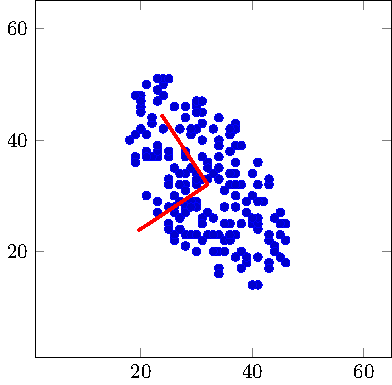
\includegraphics[width=\textwidth]{Images/PCA_Sample.pdf}
	 \end{figure}
   \end{columns}
 \end{frame}

 \begin{frame}{Dealing with an Image Stack}
   \begin{columns}
	 \column{.5\textwidth}
	 \begin{figure}[ht!]
	   \centering
	   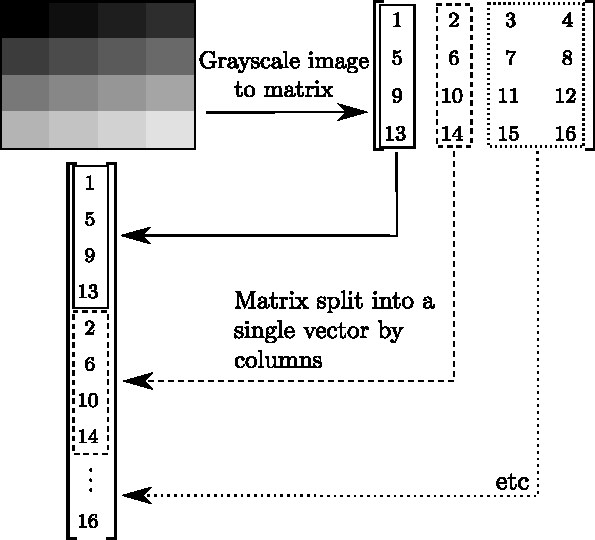
\includegraphics[width=\textwidth]{Images/pca_frame_decomposition.pdf}
	 \end{figure}
	 \column{.5\textwidth}
	 \begin{figure}[ht!]
	   \centering
	   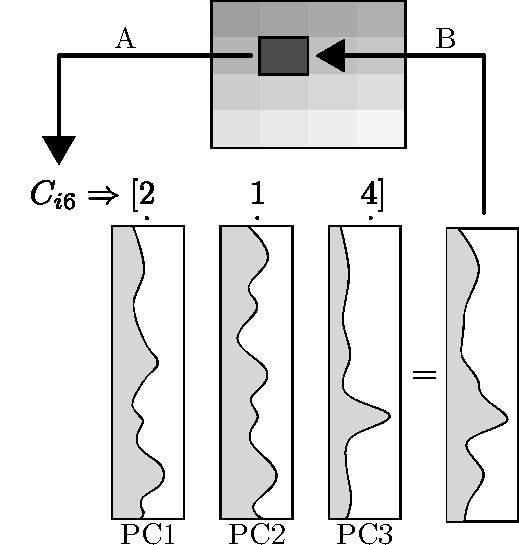
\includegraphics[width=\textwidth]{Images/pca_linearcombo.pdf}
	 \end{figure}
   \end{columns}
 \end{frame}

 \begin{frame}{PCA Effectiveness}
   \begin{columns}
	 \column{.5\textwidth}
	 \begin{figure}[ht!]
	   \centering
	   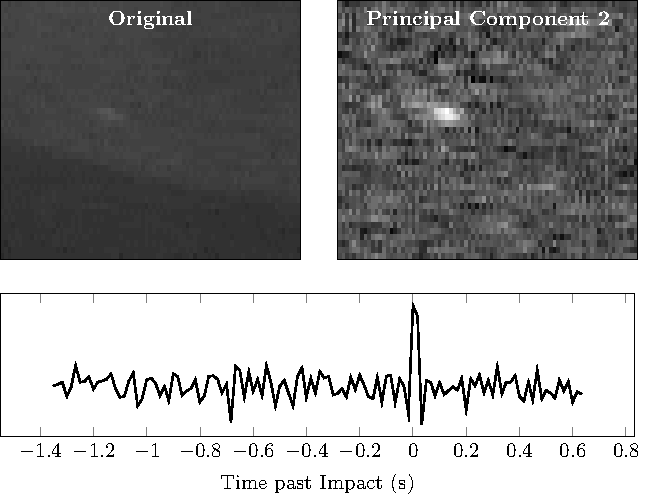
\includegraphics[width=\textwidth]{Images/pca_example2.pdf}
	 \end{figure}
	 \column{.5\textwidth}
	 \begin{itemize}
	   \item Pros:
		 \begin{itemize}
		   \item Enhanced impact image
		 \end{itemize}
	   \item Cons:
		 \begin{itemize}
		   \item Requires localized region and time
		   \item Which PC's show impact signatures can vary
		   \item Not a miracle worker
		 \end{itemize}
	 \end{itemize}
   \end{columns}
 \end{frame}

\end{document}
